\section { Parameterization of the Detector Response}

As published RMC spectra have the detector response convolved in, to compare
them to the model predictions one needs to know the detector response.

Fortunately, the TRIUMF group, which has published the most recent and highest statistics
RMC spectra, has also made published its detector response -
see \cite{RMC_1992_PhysRevC.46.1094} and \cite{RMC_1998_PhysRevC.58.1767}. 

The detector response D(E,E') is defined as the probability for a photon
with energy E to be reconstructed in the detector with energy E'. As follows from the
definition, D(E,E') includes both resolution and acceptance - the integral of D(E,E')dE'
gives the total acceptance for a given energy E.

In both \cite{RMC_1992_PhysRevC.46.1094} and \cite{RMC_1998_PhysRevC.58.1767}, the
detector response is determined using the GEANT3-based simulation using monoenergetic
photons in a energy range of 50-140 MeV, and parameterized analytically.
The parameterizations of  \cite{RMC_1992_PhysRevC.46.1094} and \cite{RMC_1998_PhysRevC.58.1767}
are significantly different, the source of the difference is not understood.

%%%%%%%%%%%%%%%%%%%%%%%%%%%%%%%%%%%%%%%%%%%%%%%%%%%%%%%%%%%%%%%%%%%%%%%%%%%%%%
\subsection { 1992 Detector response parametrization }

The response of the TRIUMF RMC spectrometer published in \cite{RMC_1992_PhysRevC.46.1094}
is described as a Gaussian function with exponential low- and  high-energy tails.
In order to reproduce the low-energy resolution tail for high-energy photons, a second Gaussian
is added for photon energies above 60 MeV. The functional form is as follows:

\begin{equation}
  \label{eq:001}
\text{D(E,E')}= \left\{
\begin{array}{ll}
                \text{A exp}\left[-\frac{1}{2\sigma_0^2}(E'-E_o)^2\right]+
                \text{F exp}\left[-\frac{1}{2\sigma_3^2}(E'-E_3)^2\right]
 \quad E_1<E'<E_2 \\
                \text{B exp}\left[-\frac{1}{\sigma_1}(E_1-E') \right]+
                \text{F exp}\left[-\frac{1}{2\sigma_3^2}(E'-E_3)^2\right]
 \quad E'<E_1      \\  
                \text{C exp}\left[-\frac{1}{\sigma_2}(E'-E_2)\right]+
                \text{F exp}\left[-\frac{1}{2\sigma_3^2}(E'-E_3)^2\right]
 \quad E'>E2     
 \end{array}
 \right\}
\end{equation}
 
where $E_1=E_0 - \frac{\sigma_0^2}{\sigma_1}$, $E_2 =E_0 + \frac{\sigma_0^2}{\sigma_2}$,
 $B=\text{A exp}\left[-\frac{\sigma_0^2}{2\sigma_1^2}\right]$, 
 $C=\text{A exp}\left[\frac{\sigma_0^2}{2\sigma_2^2}\right]$. 

 The parameters $A, B ,C , F, \sigma_i$, etc. are fitted as polynomials in the photon energy:
 
\begin{equation}
  f(E)= P_0+P_1E+P_2E^2+P_3E^3
\end{equation}

The coefficients are reported in Tables ~\ref{tab:coefficients1} and ~\ref{tab:coefficients2} .

\begin{table}[!h]
\begin{center}
\begin{tabular}{| c | c | c | c | c | }
\hline
Parameter & $P_0$ (MeV)& $P_1$ & $P_2$ (MeV)$^{-1}$ \\ \hline
$\sigma_0$ & -0.5836 & 0.0352 & \\ \hline
$\sigma_1$ & -5.879 & 0.1653 & -5.149$\times 10^{-4}$ \\ \hline
$\sigma_2$ & 1.596 & -0.03859 & 3.883$\times 10^{-4}$ \\ \hline
$\sigma_3$ & -47.80 & 1.010 & -4.406$\times 10^{-3}$ \\ \hline
E$_3$ & 1.068 & 0.7507 & \\ \hline
E$_0$ (E>60) & -1.161 & 0.9481 & 1.724$\times 10^{-3}$ \\ \hline
E$_0$ (E<60) & 22.73 & 0.1995 & 5.993$\times 10^{-3}$ \\ \hline

\end{tabular}
\end{center}
\caption{
  Polynomial parameterization of the coefficiencts in \ref{eq:001}
  \label{tab:coefficients1}}
\end{table}

\begin{table}[!h]
\begin{center}
\begin{tabular}{| c | c | c | c | c | c |}
\hline
Parameter & $P_0$ & $P_1$ (MeV)$^{-1}$ & $P_2$ (MeV)$^{-2}$  & $P_3$ (MeV)$^{-3}$\\ \hline
A & 3.259$\times 10^{-4}$ & -4.120$\times 10^{-4}$ & 1.015$\times 10^{-5}$ & -4.05$\times 10^{-8}$  \\ \hline
F/A & -0.1337 & 2.828$\times 10^{-3}$ & -9.701$\times 10^{-6}$ & \\ \hline
\end{tabular}
\end{center}
\caption{Polynomial parameterization of coefficients in \label{tab:coefficients2}}
\end{table}

The energy dependence of several coefficients used to parameterize the response
function is shown in Figure~\ref{fig:parameterDependence}.

\begin{figure}[!h]
  \begin{center}
    \includegraphics[width=0.33\columnwidth]{png/sigmas92.png} 
    \includegraphics[width=0.33\columnwidth]{png/A_FoverA92.png} 
    \includegraphics[width=0.33\columnwidth]{png/E092.png} 
  \end{center}
  \caption{
    Energy dependence of parameters defining the TRIUMF RMC spectrometer response
    \cite{RMC_1992_PhysRevC.46.1094}
  }
  \label{fig:parameterDependence}
\end{figure}

Examples of the detector response at different energies, namely, \mbox{50 MeV},
70 MeV , 90 MeV, and 110 MeV, are shown in Figure~\ref{fig:92ResponseExample}.

As previously described, for photon energies above 60 MeV, the low-energy tails are well evident.

\begin{figure}[!h]
\centering
\includegraphics[width =\textwidth]{png/Resp_example92.png}
\caption{1992 detector response parametrization for different photon energies}
\label{fig:92ResponseExample}
\end{figure}


\subsection { 1998 Detector Response }

The TRIUMF RMC spectrometer response published in 1998 (\cite{RMC_1998_PhysRevC.58.1767})
is significantly different from its 1992 version.
The 1998 parameterization is a Gaussian with logaritmic low-energy and exponential
high-energy tails:

\begin{equation}
  D(E,E')= \left\{
    \begin{array}{ll}
      \beta \cdot ln(x)/x    \qquad E' \leq (E_0-\sigma_0) \\
      Ae^{-(E'-E_0)^2/2\sigma_0^2} \qquad E_0-\sigma_0<E'<(E_0-\sigma_0^2/\sigma^2) \\
      Ae^{-(E'-E_0)/2\sigma_2}    \qquad E' \geq (E_0+\sigma_0^2/\sigma_2)
    \end{array}
  \right\}
\end{equation}

The parameter $\beta$  allows matching of the low-side and the Gaussian core
of the distribution at E'=$E_0-\sigma_0$.
$x$ is defined as
$$
  x= \frac{\alpha- E'}{\alpha -37} 
$$, with E' in MeV.
Dependence of the coefficients $\alpha, A, E_0, \sigma_0, \sigma_2$ on the photon energy
is parameterized with the 3-rd order polinomials:

\begin{equation}
  \alpha= a_0+a_1y+a_2y^2+a_3y^3
\end{equation}

where $y= (E-60)/60$, with E in MeV.

Polinomial coefficients which parameterize the energy dependence of
$\alpha, A, E_0, \sigma_0, \sigma_2$ are presented in Table~\ref{tab:param98}

\begin{table}[!h] \label{tab:param98}
  \begin{center}
    \begin{tabular}{| c | c | c | c | c | c | }
      \hline
      Parameter  & $a_0$              & $a_1$ & $a_2$ & $a_3$ \\ \hline
      $\alpha$   & 56.1               &62.5 & -0.826 & 0.0  \\ \hline
      A          & 9.41$\cdot 10^{-4}$ & 2.61$\times 10^{-3}$ &0.27 $\times 10^{-2}$ &0.835$\times 10^{-3}$   \\ \hline
      $E_0$      & 54.4               & 57.7 & -0.315 &0.0 \\ \hline
      $\sigma_0$ & 2.03               &10.4 &1.25 & -0.428\\ \hline
      $\sigma_2$ & 0.786              & 0.508 & 0.425 & -0.164\\ \hline
    \end{tabular}
  \end{center}
  \caption{Coefficients used to parameterize the energy dependence of the response function parameters}
\end{table}

Figure~\ref{fig:parameters98} shows the energy dependence of the coefficients used
in the detector response function parameterization.

\begin{figure}[!h]
  \begin{center}
    \includegraphics[width=0.49\columnwidth]{png/sigmas98.png} 
    \includegraphics[width=0.49\columnwidth]{png/par98.png} 
  \end{center}
  \caption{Energy dependence of the different parameter defining the detector response}
  \label{fig:parameters98}
\end{figure}

Figure~\ref{fig:response98} shows the 1998 detector response for the same four photon energies as shown in Figure~\ref{fig:92ResponseExample}.

The distributions in Figure~\ref{fig:response98} are significantly wider than similar distributions
shown in Figure~\ref{fig:92ResponseExample}. Given that there were no big reported changes in the TRIUMF
RMC spectrometer configuration, one can conclude that understanding of the detector response has
significantly evolved in between 1992 and 1998. However, there is no corresponding discussion 
in the 1998 paper. 

\begin{figure}[!h]
\centering
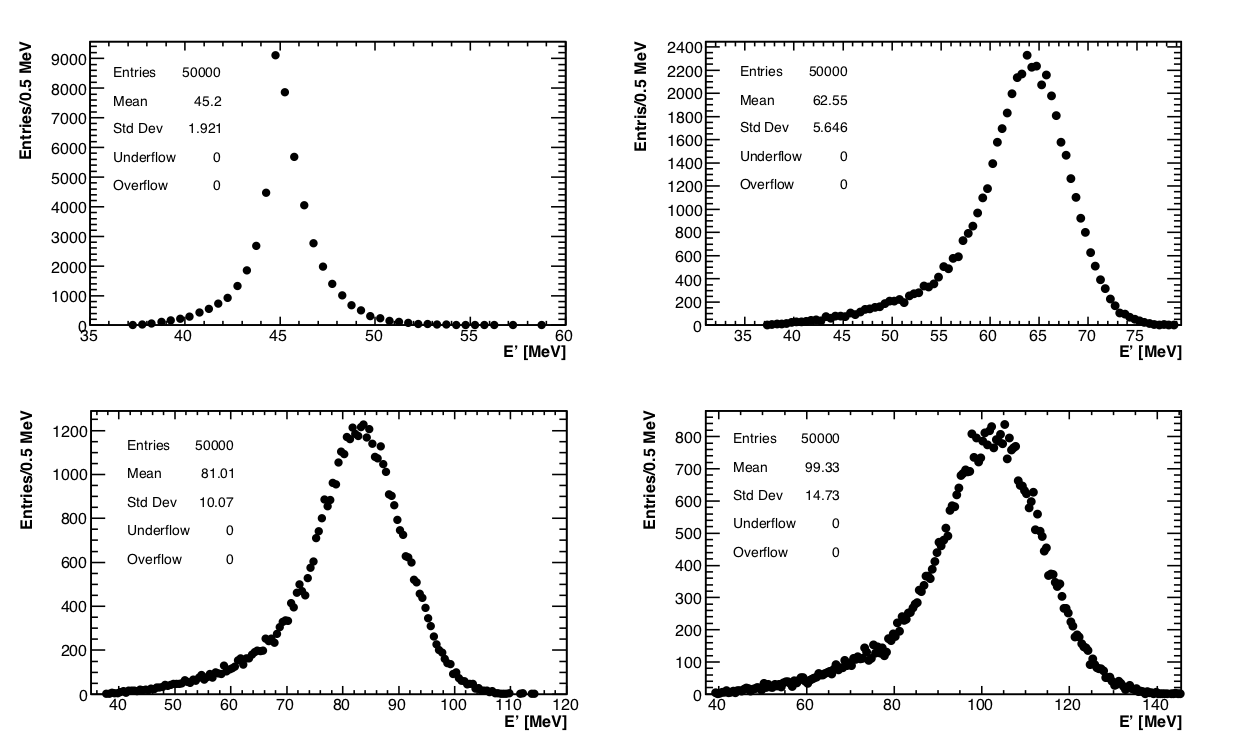
\includegraphics[width =\textwidth]{png/Resp_example98.png}
\caption{1998 detector response parametrization for different photon energies}
\label{fig:response98}
\end{figure}

Figure~\ref{fig:shapecomp} compares the 1992 and 1998 versions of the
TRIUMF RMC spectrometer response at E = 90 MeV (left) and 
the linearity of the detector response for 1992 and 1998 version
as a function of the photon energy (right).

\begin{figure} [!h]
\centering
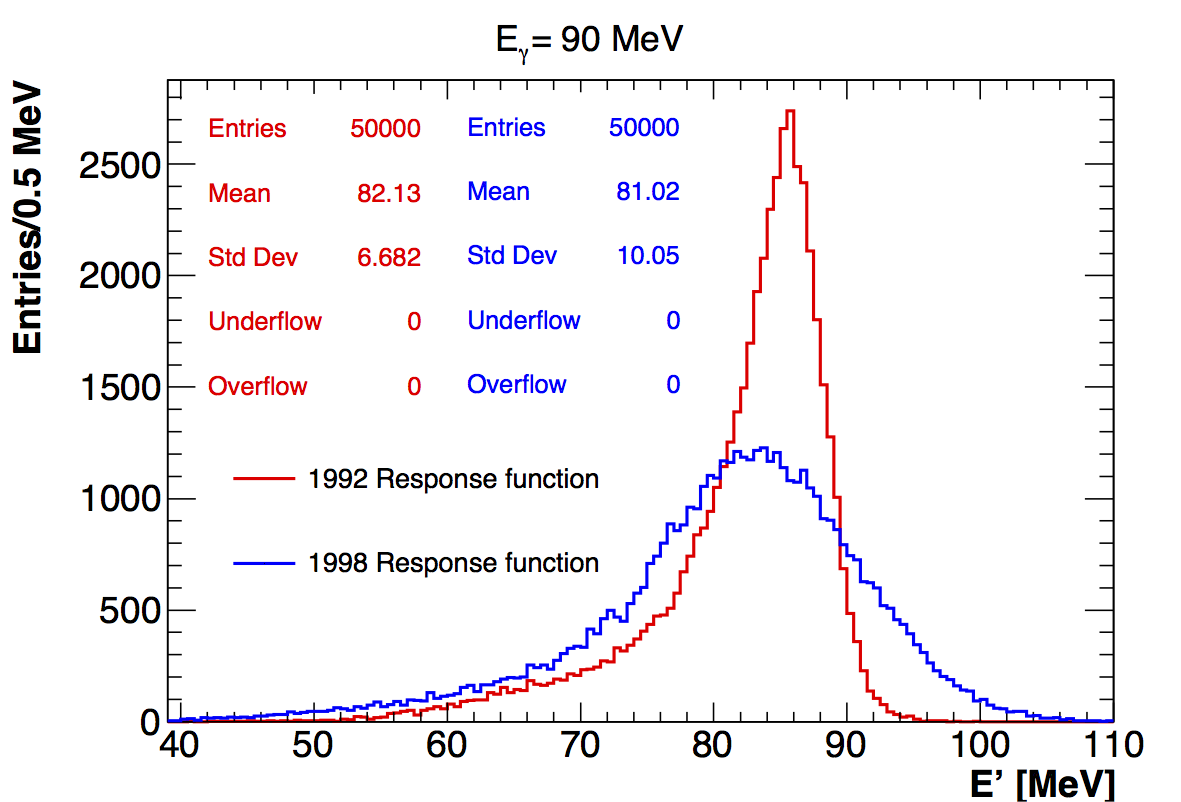
\includegraphics[width=0.49\columnwidth]{png/detRespinsieme.png}
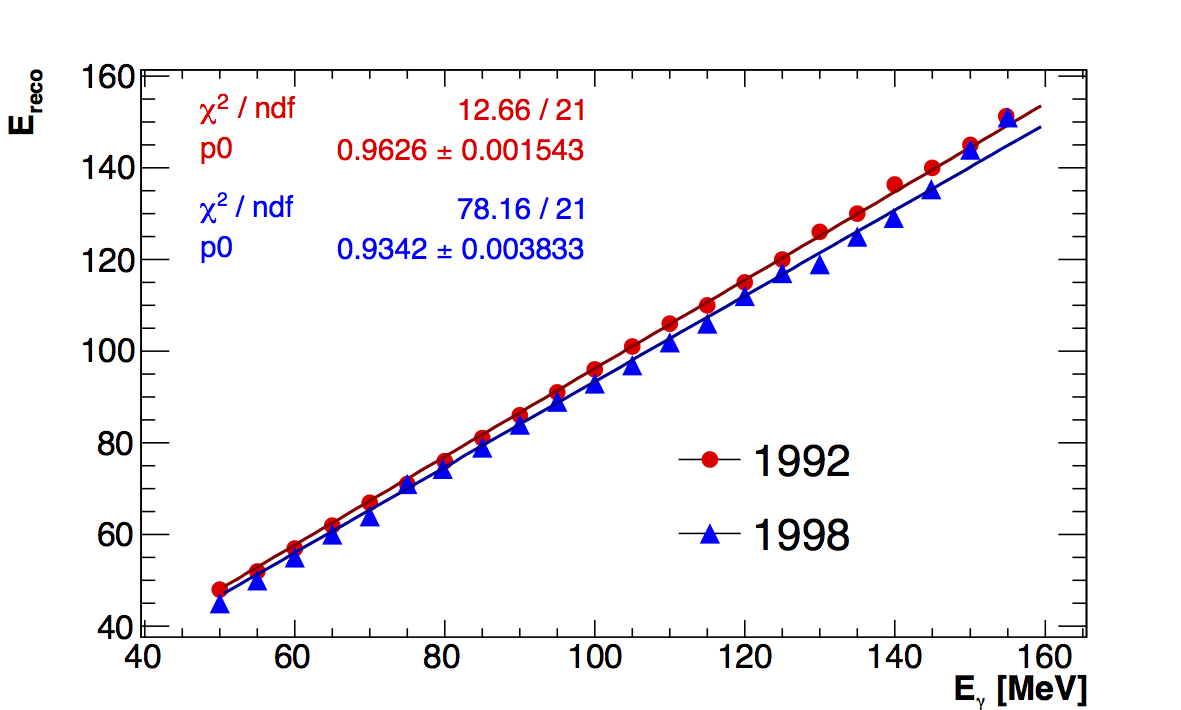
\includegraphics[width=0.49\columnwidth]{png/9298fit.png}
\caption{
  Left: 1992 and 1998 detector response at $E_{\gamma}=90$ MeV.
  Right: dependence of the peak of the detector response function on $E_{\gamma}$
  for 1992 and 1998 response parameterizations.
}
\label{fig:shapecomp} 
\end{figure}

Figure ~\ref{p004} shows how well the 1992 and 1998 parameterizations of the detector
response describe the radiative pion capture (RPC) peak on hydrogen at E = 129.4 MeV
from $\pi^{-}p \rightarrow \gamma n$ on LH$_{2}$ reaction reported in the 1992 paper.
Figure ~\ref{p004} demonstrates that the modeled 1992 detector response is consistent
with the 1992 data, and the difference between the two parameterizations can't be
interpreted in terms of an improved, from 1992 to 1998, understanding of the detector
response.\\

  \begin{figure}[!h]
 \begin{center}
 \includegraphics[width=0.49\columnwidth]{png/RPC_Data_vs_1992_Response.png} 
 \includegraphics[width=0.49\columnwidth]{png/RPC_Data_vs_1998_Response.png} 
 \end{center}
 \caption{Response function of the 1992 article (left) and 1998 article (right) compared with the 129.4 MeV line from RPC on LH$_{2}$}
 \label{p004}
 \end{figure}

 The 1998 article also validates the detector response, showing the MC description of the
 photon spectrum from RPC on $^{12}$Ca  - see Figure~\ref{fig:art9}. However, this distribution
 is wide so the 1998 data-to-MC comparison is less sensitive to the modeled detector resolution
 than the 1992 comparison.

\begin{figure}[!h]
 \begin{center}
 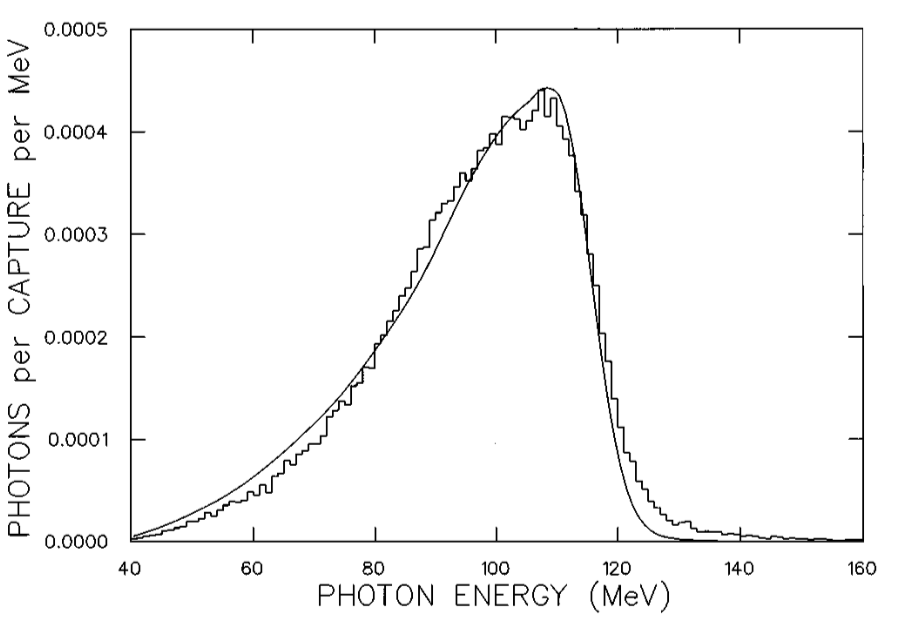
\includegraphics[width=0.45\textwidth]{png/RPC12Ca.png} 
 \end{center}
 \caption{RPC spectrum from  $\pi^{-}p \rightarrow \gamma n$ on  $^{12}$Ca compared to the simulated data }
 \label{fig:art9}
 \end{figure}
